In the registration process, the metric typically compare intensity values 
in the fixed image with the corresponding values in the transformed moving
image. When a point is mapped from one space to another by a transform,
it will in general be mapped to a non-grid position. Therefore, interpolation
is required to evaluate the image intensity at the mapped position.

\begin{figure}
\center
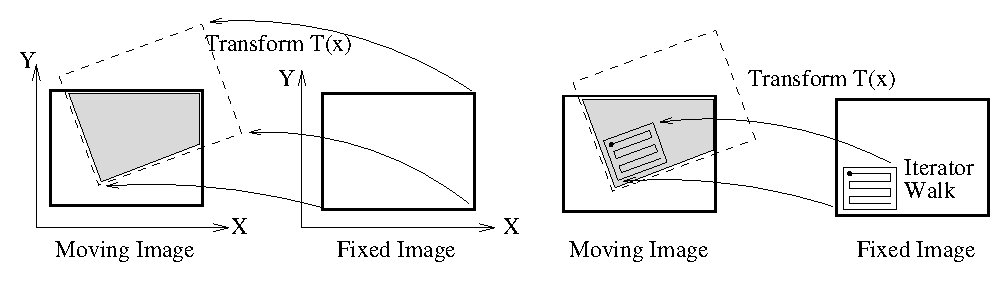
\includegraphics[height=6cm]{ImageOverlap.eps}
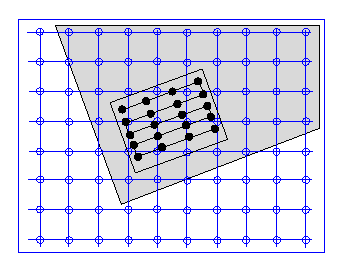
\includegraphics[height=6cm]{ImageOverlapInterpolator.eps}
\caption{ The moving image is mapped into the fixed image space under some spatial
transformation. Grid positions of the fixed image maps to non-grid positions of the
moving image. Interpolation is needed for estimating the intensity of the
moving image at these non-grid positions.}
\label{fig:ImageOverlapInterpolator}
\end{figure}

ITK currently offers three different interpolation schemes: nearest-neighbor,
linear and B-Spline. In the context of registration, the interpolation method
affects the smoothness of the optimization search space and the overall
computation time. On the other hand, interpolations are executed thousands of
times in a single optimization cycle. Hence, the user has to tradeoff the
simplicity of computation with smoothness when selecting the interpolation 
scheme.
 
\subsection{Nearest Neighbor Interpolation}
\label{sec:NearestNeighborInterpolation}
The nearest-neighbor interpolation scheme simply use the intensity of
the nearest grid position. That is, it assumes that the image intensity
is piecewise constant with jumps mid-way between grid positions. 
This interpolation scheme is cheap as it does not require any 
floating point computations.

\subsection{Linear Interpolation}
\label{sec:LinearInterpolation}
This interpolation scheme assumes that intensity varies linearly
between grid positions. Unlike nearest neighbor, the interpolated
intensity is spatially continuous. However, the intensity gradient
will be discontinous at grid positions.

\subsection{B-Spline Interpolation}
\label{sec:BSplineInterpolation}
This scheme represents the image intensity using B-Spline basis functions.
When an input image is first connected to the interpolator, B-Spline 
coefficients are computed using recursive filtering (assuming mirror
boundary conditions). Intensity at a non-grid position is computed
by multiplying the B-Spline coefficients with shifted B-Spline kernels
within a small support region of the requested position.

Currently, \code{BSplineInterpolateImageFunction} support spline order
from 0 to 5. Spline order of 0 is almost identical to nearest-neighbor.
Spline order of 1 is exactly identical to linear interpolation. For 
spline order greater than 1, both the interpolated value and their
derivative are spatially continuous.

It is important to note that when using this scheme, the interpolated
value may lie outside the range of input image intensity. This is
especially important when handling unsigned data, as it is possible
that the interpolated value to be negative.


